\chapter{Implementace}
\label{chap:implementation}

\section{Server}

Serverová část aplikace je napsána v Pythonu. To je jediná rozumná možnost, protože Mozaik je Pythonový framework a bez něj není možné číst data z datastore. Vzhledem k tomu, že potřebujeme jenom jednoduchý lightweight server pro datové API, zvolili jsme framework Flask, který je pro podobné servery populární volbou.

Server je optimalizovaný pro využití jedním uživatelem naráz. To odpovídá předpokládaným scénářům použití, kdy je buď server nasazen na lokálním stroji, nebo využíván malou skupinou výzkumníků. Poslední datastore instance načtená pomocí Mozaiku zůstává cachovaná v paměti dokud není požadován jiný datastore.

\section{Webový klient}

Nejprve je nutné přiblížit si konkrétní použité technologie a jejich principy.

\subsection{Angular}

Webový klient je vyvíjen ve frameworku Angular\footnote{\url{https://angular.io/}}. Tato volba je podložena řadou argumentů:

\begin{enumerate}
  \item Angular slouží k vývoji SPA (Single Page Application). To je pro nás klíčová funkce, protože si nemůžeme dovolit opakované načítání stejných dat ze serveru.
  \item Angular je aktivně vyvíjen společností Google, která ho sama intenzivně využívá. To je přesvědčivá odpověď na požadavek na framework, který tu ještě nějakou dobu bude.
  \item Angular směřuje vývojáře k vývoji na základě specifických konvencí. Ty vedou k škálovatelnému a udržitelnému kódu. Kromě toho je primárním jazykem Angularu Typescript, který přináší svým statickým typováním stejné výhody.
\end{enumerate}

\subsubsection*{Komponentová architektura}

Angular je založen na komponentové architektuře. Základní stavební blok je komponenta, která se skládá ze tří částí.

\begin{description}
  \item[Typescriptová třída]
  \item[Template] je psán v jazyce specifickém pro Angular, jenž je nadstavbou nad HTML, která umožňuje do kódu přidávat podmínky, cykly a zobrazovat data typescriptové třídy. Angular sleduje stav aplikace a automaticky podle něj aktualizuje renderované HTML. Za tuto funkčnost je zodpovědný sofistikovaný a vysoce optimalizovaný change detector.
  \item[Styly] jsou ve výsledném css souboru specifikovány právě pro danou komponentu, takže neovlivňují jiné komponenty.
\end{description}

Kromě komponent sev Angularu používají ještě directives, které nespecifikují vlastní template a styly, ale naváží se na již existující HTML elementy. Příkladem může být například directive, které zvýrazní svůj hostující element při kliknutí. Posledním základním kamenem jsou services, které s výsledným HTML neinteragují vůbec. Services mohou například komunikovat se serverem.

Všechny tři typy tříd mohou využívat dependency injection. Díky tomu je snadné získat například referenci na nějaký důležitý service, nebo na hostující element v případě directive.

\begin{exmp}
  Příklad Angularové komponenty, která po svém vytvoření načte a zobrazí data ze serveru.

  \begin{lstlisting}
    @Component({
      selector: 'test-component',
      template: `
        <span
          class="name"
          *ngFor="let name of names$ | async"
        >
          {{name}}
        <span>
      `
    })
    class TestComponent implements OnInit {
      names$: Observable<string[]>;

      constructor(private namesS: NamesService) {}

      ngOnInit() {
        this.names$ = this.namesS.loadData();
      }
    }
  \end{lstlisting}

  Komponenta získá při vytvoření pomocí dependency injection referenci na service, která umí ze serveru získat seznam jmen. Po jejich načtení pro každé jméno vyrenderuje jeden \lstinline|span| element. O tom, co je to \lstinline|Observable|, si povíme za chvíli.
\end{exmp}

\subsubsection*{Tok dat}

Komponenty a directives si mezi sebou mohou předávat data buď shora dolu, nebo zezdola nahoru. Shora dolu je to velice jednoduché, zkrátka se v templatu nastaví atribut elementu. Zezdola nahoru se data předávají vyvoláváním eventů.

\begin{exmp}
  Příklad Angularové komponenty, která komunikuje se svým potomkem

  \begin{lstlisting}
    @Component({
      selector: 'child',
      template: ''
    })
    class Child {
      @Input() propA: number;
      @Output() propB = new EventEmitter<number>();
    }

    @Component({
      selector: 'parent',
      template: `
        <child
          [propA]="1"
          (propB)="childVal = $event"
        ></child>
      `
    })
    class Parent {
      childVal: number;
    }
  \end{lstlisting}

  Komponenta \/\lstinline|Parent| nastaví \/\lstinline|Child| property \/\lstinline|propA| na 1. Při vyvolání \/\lstinline|propB| eventu se spustí handler, který nastaví \/\lstinline|Parent.childVal| na novou hodnotu.
\end{exmp}

Předávání dat na větší vzdálenosti, než je jen rodič a dítě, se dá řešit například pomocí services. Ve větší aplikaci je ale potřeba řídit tok dat systematicky. V Angularu se pro tento úkol používá state management knihovna NgRx. Ta silně využívá (stejně jako Angular) knihovnu RxJS. Nejprve si tedy představíme ji.

\subsection{RxJS}

RxJS\footnote{\url{https://rxjs.dev/}} je alternativa oproti callbackům nebo promisům využívající principů reaktivního programování. Hlavní roli zde má \emph{observable}, což je objekt, který (většinou asynchronně) produkuje hodnoty. Observables lze všelijak kombinovat, filtrovat, nebo transformovat. Zároveň jsou ve výchozím stavu lazy evaluated.

\begin{exmp}
  Příklad observable DOM událostí a různých operátorů. Observable začne poslouchat kliknutí na tlačítko až po zavolání \/\lstinline|subscribe|.

  \begin{lstlisting}[language=c++]
    fromEvent(myButton, 'click').pipe(
      auditTime(100), // ignoruj hodnoty po 100 ms
      // a pak vysli posledni z nich
      take(5), // prvnich 5 hodnot
      filter((event, i) => i % 2 == 0), // sude
      
      // pro kazdou udalost odesli dotaz
      // na server a dal vysilej data
      // ze serveru (getData vraci Observable)
      mergeMap(() => httpService.getData())
    ).subscribe(
      data => console.log('server response', data)
    );
  \end{lstlisting}
\end{exmp}

\subsection{NgRx}

Ngrx\footnote{\url{https://ngrx.io/}} se stará o globální stav aplikace.

\subsubsection*{Store}

Store je úložiště pro globální stav. Aplikace je o změnách jeho částí notifikována prostřednictvím observables. Stav je imutabilní, musí se vždy nahradit celý. Tento proces se neděje přímočaře, ale pomocí akcí a reducerů.

\subsubsection*{Action}

Action je popis činnosti, kterou se mění stav. V aplikaci je definováno velké množství pojmenovaných akcí. Ty mohou být odkudkoli vyvolány. Akce má jméno a volitelně ještě nějaký payload. Třeba akce \lstinline|addSelectedNeuron| může mít jako payload id neuronu.

\subsubsection*{Reducer}

Reducer je funkce, která přijme stav a akci a vrátí nový stav. Reducer by měl být deterministický a neměl by mít vedlejší efekty.

\subsubsection*{Effect}

Vedlejší efekty by měly být definovány zde. Jedná se o třídu, která sleduje akce a na jejich základě něco vykoná a (většinou) vyvolá novou akci.

\begin{exmp}
  Jak by mohla vypadat sekvence při přihlášení uživatele?

  \begin{enumerate}
    \item Komponenta \/\lstinline|LoginDialog| vyvolá akci \/\lstinline|login({username, password})|
    \item Reducer zpracuje akci a vrátí nový stav, kde \/\lstinline|userLoading = true|
    \item \lstinline|LoginDialog| je notifikován o novém stavu a zobrazí spinner
    \item Efekt \/\lstinline|AuthEffects| si všimne akce a zavolá \\\lstinline|AuthService.verifyUser(username, password)|
    \item Server potvrdí správnost jména a hesla
    \item \lstinline|AuthEffects| vyvolá akci \/\lstinline|loggedIn({userData})|
    \item Reducer zpracuje akci a vrátí nový stav, kde \/\lstinline|userLoading = false|\\a \/\lstinline|user = userData|
    \item \lstinline|LoginDialog| je notifikován o novém stavu a zavře se
    \item Komponenta \/\lstinline|AppShell| je notifikována o novém stavu a zobrazí uvítací zprávu
  \end{enumerate}
\end{exmp}

\subsection{D3.js}

D3.js\footnote{\url{https://d3js.org/}} je knihovna pro vizualizaci dat. Její přístup je nízkoúrovňový --- místo hotových grafů nabízí dynamický přístup k SVG nebo canvas na základě dat. Poskytuje řadu klíčových prvků, jako jsou interpolátory, osy nebo matematické funkce. Je tedy ideální pro naše účely, kde potřebujeme vizualizace hodně upravovat a přidávat jim interaktivitu. Příklad zde uvádět nebudeme, protože i na obyčejný graf jsou v d3.js potřeba desítky až stovky řádek kódu.

\subsection{AlaSQL}

AlaSQL\footnote{\url{https://github.com/AlaSQL/alasql}} je in-memory SQL databáze implementovaná v Javascriptu. Podporuje velkou část standardu SQL-99, kromě toho má rozšíření pro práci s JSON nebo grafovými daty. Je to jediný projekt svého druhu a podobného měřítka. Bohužel její architektura není moc propracovaná a kód je špatně udržovatelný \cite{AlaSQLIssue}. Kvůli tomu je obtížné opravovat její stávající bugy, kterých není málo, a pravděpodobně se nelze vyvarovat bugům budoucím. V aplikaci ale využíváme pouze dotazovací část knihovny, jejíž stav pro naše potřeby dostačuje.

\subsection{Stav klienta}

Veškeré akce, reducery a efekty se nachází ve složce \lstinline|frontend/src/app/store|. Protože ADS nemají v datastore přiřazený jiný unikátní identifikátor, než je kombinace jejich základních parametrů, frontend je uchovává seřazené a identifikuje je jejich indexy.

\begin{description}
  \item[UI] je část stavu mající na starost uživatelské rozhraní. V tuto chvíli zde jsou jen nastavení pro různé překryvy.
  \item[Network] drží informace o probíhajících síťových dotazech. Uživatelé mají možnost dotazy vidět a případě zrušit.
  \item[Filesystem] slouží k uložení adresářové struktury, včetně toho, které složky uživatel rozbalil.
  \item[Model] je největší část stavu. Uchovává se zde struktura neuronové sítě, tj. neurony a jejich pozice v různých vrstvách a jejich odchozí spojení. Kromě toho se zde drží seznam vybraných neuronů, neuron, na kterém se zrovna nachází kurzor (ten se pak v aplikaci zvýrazní na všech místech, kde je vidět) a případně stav načítání modelu ze serveru.
  \item[ADS] je seznam všech ADS (zde jsou jen jejich základní informace), seznam načtených ADS (se všemi daty) a případně, podobně jako u modelu, stav jejich načítání ze serveru.
  \item[Navigator] obsahuje aktuální SQL dotaz.
  \item[Inspector] drží stavy jednotlivých záložek. Ty si každý vizualizační modul definuje sám a slouží většinou k uložení nastavení vizualizace. Kromě toho se zde ukládá, zda současně zobrazené vizualizace stejného typu sdílí svá nastavení.
\end{description}

Následující části globálního stavu se nachází v URL:

\begin{itemize}
  \item cesta k aktuálnímu datastore
  \item indexy aktuálně načtených ADS
  \item indexy aktuálně zobrazených ADS
  \item atribut, podle kterého jsou seskupované zobrazené ADS
\end{itemize}

\subsection{Moduly}

Kód je rozdělen do několika Angular modulů podle toho, kde všude je potřeba jej využívat.

\subsubsection*{Common}

Toto je modul pro všechny komponenty, které jsou za běhu aplikace vždy zobrazeny. Patří sem tabulka navigátoru, záložková struktura inspektoru, záhlaví stránky a podobně.

\subsubsection*{Widgets}

Kolekce často používaných komponent. Většina z nich jsou různé formulářové prvky, například input, range, nebo checkbox. Dále tu je stránkovač, podpora pro toast notifikace a kontejnery s měnitelnými rozměry.

\subsubsection*{DSPages}

Jedná se o složku modulů pro vizualizaci každé podporované ADS. Tyto moduly jsou načteny dynamicky za běhu podle toho, jaká ADS je zobrazena. Díky tomu je zmenšený objem Javascriptu, který klient musí před svým spuštěním načíst. Jak je ale vidět na obrázku \ref{fig:sourcemaps}, nejde o zásadní rozdíl. Sdílené části všech vizualizací se nachází v modulu \lstinline|DSPagesCommon|.

\begin{figure}
  \centering
  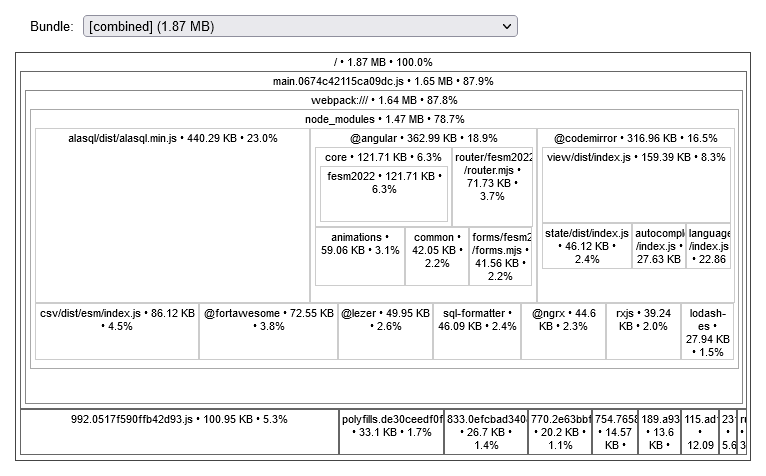
\includegraphics[width=1\linewidth]{img/sourcemaps.png}
  \caption{Rozložení minifikovaného kódu napříč webovým klientem. Je vidět, že většinu objemu tvoří knihovny třetích stran. Velikost jednotlivých dynamicky importovaných modulů (vespod vpravo) se pohybuje mezi 1.1\% až 0.02\%}
  \label{fig:sourcemaps}
\end{figure}

\subsection{SQL}

Pro snazší filtrování a transformace jsme do SQL přidali následující nestandardní funkce.

\subsubsection*{\protect\lstinline|MAKE_LINK(value)|}

Funkce očekává index ADS a vrací objekt, který se ve výsledné tabulce zobrazí jako kliknutelný odkaz na přidání ADS do inspektoru.

\subsubsection*{\protect\lstinline|JSON_STRINGIFY(value), JSON_PARSE(value)|}

Jedná se o funkce pro převod hodnot mezi JS objekty a deterministickým JSON. Hodí se například pro \lstinline|GROUP BY|, protože AlaSQL objekty porovnává podle reference.

\subsubsection*{\protect\lstinline|MAKE_INTERSECTION(value)|}
\label{sql:make_intersection}

Tato agregační funkce vrací průnik properties se stejným jménem i hodnotou ve všech poskytnutých objektech.

\begin{exmp}
  Ukázka použití \/\lstinline|MAKE_INTERSECTION| na object a na pole.

  \begin{lstlisting}[language=SQL]
    -- data: [
    --   {a: {foo: 'bar', x: 1}},
    --   {a: {foo: 'bar', x: 2}},
    -- ]

    SELECT MAKE_INTERSECTION(a) a FROM data

    -- vysledek: [
    --   {a: {foo: 'bar'}},
    -- ]

    -- data2: [
    --   {a: [1, 2, 7]},
    --   {a: [3, 7, 1, 6]},
    -- ]

    SELECT MAKE_INTERSECTION(a) a FROM data2

    -- vysledek: [
    --   {a: [1, 7]},
    -- ]
  \end{lstlisting}
\end{exmp}

\subsubsection*{SUBTRACT(minuend, subtrahend)}
\label{sql:subtract}

Fuknce, která vrací množinový rozdíl mezi první a druhou hodnotou.

\begin{exmp}
  Ukázka použití \/\lstinline|SUBTRACT| na object a na pole.

  \begin{lstlisting}[language=SQL]
    SELECT SUBTRACT(
      @{foo: 1, bar: 2, baz: 3},
      @{foo: 2, bar: 2, car: 3}
    ) a

    -- vysledek: [
    --   {a: {foo: 1, baz: 3}},
    -- ]

    SELECT SUBTRACT(
      @[1, 2, 3],
      @[4, 3, 7]
    ) a

    -- vysledek: [
    --   {a: [1, 2]},
    -- ]
  \end{lstlisting}
\end{exmp}

\subsubsection*{\protect\lstinline|MAKE_DIFF(value, diffId = 0)|}
\label{sql:make_diff}

Tato funkce není ani klasická funkce, ani agregátor. Je implementována pomocí \lstinline|MAKE_INTERSECTION| a \lstinline|SUBTRACT|, ale část z ní se musí vykonat zcela mimo AlaSQL. Více implementačních detailů je v sekcích \ref{fn:makeDiff} a \ref{comp:ds-select}.

Schová atributy se stejným jménem a hodnotou ve všech poskytnutých objektech. Je možné poskytnuté objekty oddělit pomocí \lstinline|diffId|. Tato funkce se používá například ve výchozím výpisu ADS, kde se zobrazují odlišné hodnoty ve stimulech se stejným jménem (\lstinline|MAKE_DIFF(stimulus, stimulus->name)|).

\begin{exmp}
  Ukázka použití \/\lstinline|MAKE_DIFF| na object a na pole.

  \begin{lstlisting}[language=SQL]
    -- data: [
    --   {a: {foo: 'bar', x: 1}},
    --   {a: {foo: 'bar', x: 2}},
    -- ]

    SELECT MAKE_DIFF(a) a FROM data

    -- vraci: [
    --   {a: {x: 1}},
    --   {a: {x: 2}},
    -- ]

    -- data2: [
    --   {a: [1, 2, 7]},
    --   {a: [3, 7, 1, 6]},
    -- ]

    SELECT MAKE_DIFF(a) a FROM data2

    -- vraci: [
    --   {a: [2]},
    --   {a: [3, 6]},
    -- ]

    -- data3: [
    --   {a: {foo: 'bar', x: 1}},
    --   {a: {foo: 'bar', x: 2}},
    --   {a: {foo: 'cow', x: 1}},
    --   {a: {foo: 'cow', x: 2}},
    -- ]

    SELECT MAKE_DIFF(a, a->foo) a FROM data3

    -- vraci: [
    --   {a: {x: 1}},
    --   {a: {x: 2}},
    --   {a: {x: 1}},
    --   {a: {x: 2}},
    -- ]
  \end{lstlisting}
\end{exmp}
